\protect\hyperlink{main-nav}{≡} \protect\hyperlink{close-nav}{×}

\hypertarget{section-2.3-the-power-and-sum-rules-for-derivatives}{%
\section{Section 2.3: The Power and Sum Rules for
Derivatives}\label{section-2.3-the-power-and-sum-rules-for-derivatives}}

In the next few sections, we'll get the derivative rules that will let
us find formulas for derivatives when our function comes to us as a
formula. This is a very algebraic section, and you should get lots of
practice. When you tell someone you have studied calculus, this is the
one skill they will expect you to have.

To view this video please enable JavaScript, and consider upgrading to a
web browser that \href{http://videojs.com/html5-video-support/}{supports
HTML5 video}

\hypertarget{building-blocks}{%
\subsection{Building Blocks}\label{building-blocks}}

These are the simplest rules -- rules for the basic functions. We won't
prove these rules; we'll just use them. But first, let's look at a few
so that we can see they make sense.

\hypertarget{example-1}{%
\paragraph{Example 1}\label{example-1}}

Find the derivative of \textbackslash{}( y=f(x)=mx+b \textbackslash{})

This is a linear function, so its graph is its own tangent line! The
slope of the tangent line, the derivative, is the slope of the line:
\textbackslash{}{[}f'(x)=m\textbackslash{}{]}

\hypertarget{rule}{%
\paragraph{Rule:}\label{rule}}

The derivative of a linear function is its slope.

To view this video please enable JavaScript, and consider upgrading to a
web browser that \href{http://videojs.com/html5-video-support/}{supports
HTML5 video}

\hypertarget{example-2}{%
\paragraph{Example 2}\label{example-2}}

Find the derivative of \textbackslash{}( f(x)=135 \textbackslash{}).

Think about this one graphically, too. The graph of f(x) is a horizontal
line. So its slope is zero:
\textbackslash{}{[}f'(x)=0\textbackslash{}{]}

\hypertarget{rule-1}{%
\paragraph{Rule:}\label{rule-1}}

The derivative of a constant is zero.

To view this video please enable JavaScript, and consider upgrading to a
web browser that \href{http://videojs.com/html5-video-support/}{supports
HTML5 video}

\hypertarget{example-3}{%
\paragraph{Example 3}\label{example-3}}

Find the derivative of \textbackslash{}( f(x)=x\^{}2 \textbackslash{}).

Recall the formal definition of the derivative:
\textbackslash{}{[}f'(x)=\textbackslash{}lim\textbackslash{}limits\_\{h\textbackslash{}to
0\} \textbackslash{}frac\{f(x+h)-f(x)\}\{h\}.\textbackslash{}{]}

Using our function \textbackslash{}( f(x)=x\^{}2 \textbackslash{}),
\textbackslash{}( f(x+h)=(x+h)\^{}2=x\^{}2+2xh+h\^{}2 \textbackslash{}).

Then \textbackslash{}{[} \textbackslash{}begin\{align*\} f'(x)=\&
\textbackslash{}lim\textbackslash{}limits\_\{h\textbackslash{}to 0\}
\textbackslash{}frac\{f(x+h)-f(x)\}\{h\}\textbackslash{}\textbackslash{}
=\& \textbackslash{}lim\textbackslash{}limits\_\{h\textbackslash{}to 0\}
\textbackslash{}frac\{x\^{}2+2xh+h\^{}2-x\^{}2\}\{h\}\textbackslash{}\textbackslash{}
=\& \textbackslash{}lim\textbackslash{}limits\_\{h\textbackslash{}to 0\}
\textbackslash{}frac\{2xh+h\^{}2\}\{h\}\textbackslash{}\textbackslash{}
=\& \textbackslash{}lim\textbackslash{}limits\_\{h\textbackslash{}to 0\}
\textbackslash{}frac\{h(2x+h)\}\{h\}\textbackslash{}\textbackslash{} =\&
\textbackslash{}lim\textbackslash{}limits\_\{h\textbackslash{}to 0\}
(2x+h)\textbackslash{}\textbackslash{} =\& 2x
\textbackslash{}end\{align*\} \textbackslash{}{]}

From all that, we find that \textbackslash{}( f'(x)=2x
\textbackslash{}).

Luckily, there is a handy rule we use to skip using the limit:

\hypertarget{power-rule}{%
\paragraph{Power Rule}\label{power-rule}}

The derivative of \textbackslash{}( f(x)=x\^{}n \textbackslash{}) is
\textbackslash{}{[}f'(x)=nx\^{}\{n-1\}.\textbackslash{}{]}

To view this video please enable JavaScript, and consider upgrading to a
web browser that \href{http://videojs.com/html5-video-support/}{supports
HTML5 video}

To view this video please enable JavaScript, and consider upgrading to a
web browser that \href{http://videojs.com/html5-video-support/}{supports
HTML5 video}

\hypertarget{example-4}{%
\paragraph{Example 4}\label{example-4}}

Find the derivative of \textbackslash{}( g(x)=4x\^{}3 \textbackslash{})

Using the power rule, we know that if \textbackslash{}( f(x)=x\^{}3
\textbackslash{}), then \textbackslash{}( f'(x)=3x\^{}2
\textbackslash{}). Notice that \textbackslash{}(g\textbackslash{}) is 4
times the function \textbackslash{}(f\textbackslash{}). Think about what
this change means to the graph of \textbackslash{}(g\textbackslash{}) --
it's now 4 times as tall as the graph of
\textbackslash{}(f\textbackslash{}). If we find the slope of a secant
line, it will be \textbackslash{}(
\textbackslash{}frac\{\textbackslash{}Delta g\}\{\textbackslash{}Delta
x\}= \textbackslash{}frac\{4\textbackslash{}Delta
f\}\{\textbackslash{}Delta x\}
=4\textbackslash{}frac\{\textbackslash{}Delta f\}\{\textbackslash{}Delta
x\} \textbackslash{}); each slope will be 4 times the slope of the
secant line on the \textbackslash{}(f\textbackslash{}) graph. This
property will hold for the slopes of tangent lines, too:
\textbackslash{}{[}\textbackslash{}frac\{d\}\{dx\}\textbackslash{}left(4x\^{}3\textbackslash{}right)=4\textbackslash{}frac\{d\}\{dx\}\textbackslash{}left(x\^{}3\textbackslash{}right)=4\textbackslash{}cdot
3x\^{}2=12x\^{}2.\textbackslash{}{]}

\hypertarget{rule-2}{%
\paragraph{Rule:}\label{rule-2}}

Constants come along for the ride, i.e., \textbackslash{}(
\textbackslash{}frac\{d\}\{dx\}\textbackslash{}left(
kf\textbackslash{}right)=kf'.\textbackslash{})

To view this video please enable JavaScript, and consider upgrading to a
web browser that \href{http://videojs.com/html5-video-support/}{supports
HTML5 video}

Here are all the basic rules in one place.

\hypertarget{derivative-rules-building-blocks}{%
\paragraph{Derivative Rules: Building
Blocks}\label{derivative-rules-building-blocks}}

In what follows, \textbackslash{}(f\textbackslash{}) and
\textbackslash{}(g\textbackslash{}) are differentiable functions of
\textbackslash{}(x\textbackslash{}).

\hypertarget{constant-multiple-rule}{%
\subparagraph{Constant Multiple Rule}\label{constant-multiple-rule}}

\textbackslash{}{[} \textbackslash{}frac\{d\}\{dx\}\textbackslash{}left(
kf\textbackslash{}right)=kf'\textbackslash{}{]}

\hypertarget{sum-and-difference-rule}{%
\subparagraph{Sum and Difference Rule}\label{sum-and-difference-rule}}

\textbackslash{}{[}\textbackslash{}frac\{d\}\{dx\}\textbackslash{}left(f\textbackslash{}pm
g\textbackslash{}right)=f' \textbackslash{}pm g'\textbackslash{}{]}

\hypertarget{power-rule-1}{%
\subparagraph{Power Rule}\label{power-rule-1}}

\textbackslash{}{[}\textbackslash{}frac\{d\}\{dx\}\textbackslash{}left(x\^{}n\textbackslash{}right)=nx\^{}\{n-1\}\textbackslash{}{]}

Special cases:
\textbackslash{}{[}\textbackslash{}frac\{d\}\{dx\}\textbackslash{}left(k\textbackslash{}right)=0
\textbackslash{}quad \textbackslash{}text\{(Because \textbackslash{}(
k=kx\^{}0 \textbackslash{}).)\}\textbackslash{}{]}
\textbackslash{}{[}\textbackslash{}frac\{d\}\{dx\}\textbackslash{}left(x\textbackslash{}right)=1
\textbackslash{}quad \textbackslash{}text\{(Because \textbackslash{}(
x=x\^{}1 \textbackslash{}).)\}\textbackslash{}{]}

\hypertarget{exponential-functions}{%
\subparagraph{Exponential Functions}\label{exponential-functions}}

\textbackslash{}{[}\textbackslash{}frac\{d\}\{dx\}\textbackslash{}left(e\^{}x\textbackslash{}right)=e\^{}x\textbackslash{}{]}
\textbackslash{}{[}\textbackslash{}frac\{d\}\{dx\}\textbackslash{}left(a\^{}x\textbackslash{}right)=\textbackslash{}ln(a)\textbackslash{},a\^{}x\textbackslash{}{]}

\hypertarget{natural-logarithm}{%
\subparagraph{Natural Logarithm}\label{natural-logarithm}}

\textbackslash{}{[}\textbackslash{}frac\{d\}\{dx\}\textbackslash{}left(\textbackslash{}ln(x)\textbackslash{}right)=\textbackslash{}frac\{1\}\{x\}\textbackslash{}{]}

The sum, difference, and constant multiple rule combined with the power
rule allow us to easily find the derivative of any polynomial.

To view this video please enable JavaScript, and consider upgrading to a
web browser that \href{http://videojs.com/html5-video-support/}{supports
HTML5 video}

To view this video please enable JavaScript, and consider upgrading to a
web browser that \href{http://videojs.com/html5-video-support/}{supports
HTML5 video}

\hypertarget{example-5}{%
\paragraph{Example 5}\label{example-5}}

Find the derivative of \textbackslash{}(
p(x)=17x\^{}\{10\}+13x\^{}8-1.8x+1003 \textbackslash{}).

\textbackslash{}{[} \textbackslash{}begin\{align*\}
\textbackslash{}frac\{d\}\{dx\}\textbackslash{}left(
17x\^{}\{10\}+13x\^{}8-1.8x+1003 \textbackslash{}right)=\&
\textbackslash{}frac\{d\}\{dx\}\textbackslash{}left( 17x\^{}\{10\}
\textbackslash{}right)+\textbackslash{}frac\{d\}\{dx\}\textbackslash{}left(
13x\^{}8
\textbackslash{}right)-\textbackslash{}frac\{d\}\{dx\}\textbackslash{}left(
1.8x
\textbackslash{}right)+\textbackslash{}frac\{d\}\{dx\}\textbackslash{}left(
1003 \textbackslash{}right)\textbackslash{}\textbackslash{} =\&
17\textbackslash{}frac\{d\}\{dx\}\textbackslash{}left( x\^{}\{10\}
\textbackslash{}right)+13\textbackslash{}frac\{d\}\{dx\}\textbackslash{}left(
x\^{}8
\textbackslash{}right)-1.8\textbackslash{}frac\{d\}\{dx\}\textbackslash{}left(
x
\textbackslash{}right)+\textbackslash{}frac\{d\}\{dx\}\textbackslash{}left(
1003 \textbackslash{}right)\textbackslash{}\textbackslash{} =\&
17\textbackslash{}left(10x\^{}9\textbackslash{}right)+13\textbackslash{}left(8x\^{}7\textbackslash{}right)-1.8\textbackslash{}left(1\textbackslash{}right)+0\textbackslash{}\textbackslash{}
=\& 170x\^{}9+104x\^{}7-1.8 \textbackslash{}end\{align*\}
\textbackslash{}{]}

You don't have to show every single step. Do be careful when you're
first working with the rules, but pretty soon you'll be able to just
write down the derivative directly:

\hypertarget{example-6}{%
\paragraph{Example 6}\label{example-6}}

Find
\textbackslash{}(\textbackslash{}frac\{d\}\{dx\}\textbackslash{}left(
17x\^{}2-33x+12 \textbackslash{}right)\textbackslash{}).

Writing out the rules, we'd write
\textbackslash{}{[}\textbackslash{}frac\{d\}\{dx\}\textbackslash{}left(
17x\^{}2-33x+12
\textbackslash{}right)=17(2x)-33(1)+0=34x-33.\textbackslash{}{]}

Once you're familiar with the rules, you can, in your head, multiply the
2 times the 17 and the 33 times 1, and just write
\textbackslash{}{[}\textbackslash{}frac\{d\}\{dx\}\textbackslash{}left(
17x\^{}2-33x+12 \textbackslash{}right)=34x-33.\textbackslash{}{]}

The power rule works even if the power is negative or a fraction. In
order to apply it, first translate all roots and basic rational
expressions into exponents:

\hypertarget{example-7}{%
\paragraph{Example 7}\label{example-7}}

Find the derivative of \textbackslash{}(
y=3\textbackslash{}sqrt\{t\}-\textbackslash{}frac\{4\}\{t\^{}4\}+5e\^{}t
\textbackslash{}).

The first step is translate into exponents:
\textbackslash{}{[}y=3\textbackslash{}sqrt\{t\}-\textbackslash{}frac\{4\}\{t\^{}4\}+5e\^{}t=3t\^{}\{1/2\}-4t\^{}\{-4\}+5e\^{}t\textbackslash{}{]}

Now you can take the derivative: \textbackslash{}{[}
\textbackslash{}begin\{align*\}
\textbackslash{}frac\{d\}\{dt\}\textbackslash{}left(
3t\^{}\{1/2\}-4t\^{}\{-4\}+5e\^{}t \textbackslash{}right)=\&
3\textbackslash{}left(\textbackslash{}frac\{1\}\{2\}t\^{}\{-1/2\}\textbackslash{}right)-4\textbackslash{}left(-4t\^{}\{-5\}\textbackslash{}right)+5\textbackslash{}left(e\^{}t\textbackslash{}right)
\textbackslash{}\textbackslash{} =\&
\textbackslash{}frac\{3\}\{2\}t\^{}\{-1/2\}+16t\^{}\{-5\}+5e\^{}t
\textbackslash{}end\{align*\} \textbackslash{}{]}

If there is a reason to, you can rewrite the answer with radicals and
positive exponents: \textbackslash{}{[}y'=
\textbackslash{}frac\{3\}\{2\}t\^{}\{-1/2\}+16t\^{}\{-5\}+5e\^{}t=
\textbackslash{}frac\{3\}\{2\textbackslash{}sqrt\{t\}\}+\textbackslash{}frac\{16\}\{t\^{}5\}+5e\^{}t\textbackslash{}{]}

Be careful when finding the derivatives with negative exponents.

We can immediately apply these rules to solve the problem we started the
chapter with - finding a tangent line.

\hypertarget{example-8}{%
\paragraph{Example 8}\label{example-8}}

Find the equation of the line tangent to \textbackslash{}(
g(t)=10-t\^{}2 \textbackslash{}) when \textbackslash{}(t =
2\textbackslash{}).

The slope of the tangent line is the value of the derivative. We can
compute \textbackslash{}( g'(t)=-2t \textbackslash{}). To find the slope
of the tangent line when \textbackslash{}(t = 2\textbackslash{}),
evaluate the derivative at that point. The slope of the tangent line is
-4.

To find the equation of the tangent line, we also need a point on the
tangent line. Since the tangent line touches the original function at
\textbackslash{}(t = 2\textbackslash{}), we can find the point by
evaluating the original function: \textbackslash{}( g(2)=10-2\^{}2=6
\textbackslash{}). The tangent line must pass through the point (2, 6).

Using the point-slope equation of a line, the tangent line will have
equation \textbackslash{}( y-6=-4(t-2) \textbackslash{}). Simplifying to
slope-intercept form, the equation is \textbackslash{}( y=-4t+14
\textbackslash{}).

Graphing, we can verify this line is indeed tangent to the curve:

\begin{figure}
\centering
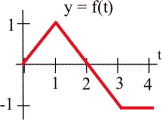
\includegraphics{images/image036.png}
\caption{}
\end{figure}

We can also use these rules to help us find the derivatives we need to
interpret the behavior of a function.

\hypertarget{example-9}{%
\paragraph{Example 9}\label{example-9}}

In a memory experiment, a researcher asks the subject to memorize as
many words from a list as possible in 10 seconds. Recall is tested, then
the subject is given 10 more seconds to study, and so on. Suppose the
number of words remembered after \textbackslash{}(t\textbackslash{})
seconds of studying could be modeled by \textbackslash{}(
W(t)=4t\^{}\{2/5\} \textbackslash{}). Find and interpret
\textbackslash{}( W'(20) \textbackslash{}).

\textbackslash{}( W'(t)=4\textbackslash{}cdot
\textbackslash{}frac\{2\}\{5\}t\^{}\{-3/5\}=\textbackslash{}frac\{8\}\{5\}t\^{}\{-3/5\}
\textbackslash{}), so \textbackslash{}(
W'(20)=\textbackslash{}frac\{8\}\{5\}(20)\^{}\{-3/5\}\textbackslash{}approx
0.2652 \textbackslash{}).

Since \textbackslash{}(W\textbackslash{}) is measured in words, and
\textbackslash{}(t\textbackslash{}) is in seconds,
\textbackslash{}(W'\textbackslash{}) has units words per second.
\textbackslash{}( W'(20)\textbackslash{}approx 0.2652 \textbackslash{})
means that after 20 seconds of studying, the subject is learning about
0.27 more words for each additional second of studying.

\hypertarget{business-and-economics-terms}{%
\subsection{Business and Economics
Terms}\label{business-and-economics-terms}}

Next we will delve more deeply into some business applications. To do
that, we first need to review some terminology.

Suppose you are producing and selling some item. The profit you make is
the amount of money you take in minus what you have to pay to produce
the items. Both of these quantities depend on how many you make and
sell. (So we have functions here.) Here is a list of definitions for
some of the terminology, together with their meaning in algebraic terms
and in graphical terms.

\hypertarget{cost}{%
\paragraph{Cost}\label{cost}}

Your \textbf{cost} is the money you have to spend to produce your items.

\hypertarget{fixed-cost}{%
\paragraph{Fixed Cost}\label{fixed-cost}}

The \textbf{Fixed Cost} (\textbf{FC}) is the amount of money you have to
spend regardless of how many items you produce. FC can include things
like rent, purchase costs of machinery, and salaries for office staff.
You have to pay the fixed costs even if you don't produce anything.

\hypertarget{total-variable-cost}{%
\paragraph{Total Variable Cost}\label{total-variable-cost}}

The \textbf{Total Variable Cost} (\textbf{TVC}) for
\textbackslash{}(q\textbackslash{}) items is the amount of money you
spend to actually produce them. TVC includes things like the materials
you use, the electricity to run the machinery, gasoline for your
delivery vans, maybe the wages of your production workers. These costs
will vary according to how many items you produce.

\hypertarget{total-cost}{%
\paragraph{Total Cost}\label{total-cost}}

The \textbf{Total Cost} (\textbf{TC}, or sometimes just \textbf{C}) for
\textbackslash{}(q\textbackslash{}) items is the total cost of producing
them. It's the sum of the fixed cost and the total variable cost for
producing \textbackslash{}(q\textbackslash{}) items.

\hypertarget{average-cost}{%
\paragraph{Average Cost}\label{average-cost}}

The \textbf{Average Cost} (\textbf{AC}) for
\textbackslash{}(q\textbackslash{}) items is the total cost divided by
\textbackslash{}(q\textbackslash{}), or
\textbackslash{}(\textbackslash{}frac\{TC\}\{q\}\textbackslash{}). You
can also talk about the average fixed cost,
\textbackslash{}(\textbackslash{}frac\{FC\}\{q\}\textbackslash{}), or
the average variable cost,
\textbackslash{}(\textbackslash{}frac\{TVC\}\{q\}\textbackslash{}).

\hypertarget{marginal-cost}{%
\paragraph{Marginal Cost}\label{marginal-cost}}

The \textbf{Marginal Cost} (\textbf{MC}) at
\textbackslash{}(q\textbackslash{}) items is the cost of producing the
next item. Really, it's \textbackslash{}{[}MC(q) = TC(q + 1) -
TC(q).\textbackslash{}{]} In many cases, though, it's easier to
approximate this difference using calculus (see Example 1 below). And
some sources define the marginal cost directly as the derivative,
\textbackslash{}{[}MC(q) = TC'(q).\textbackslash{}{]} In this course, we
will use both of these definitions as if they were interchangeable.

The units on marginal cost is cost per item.

Why is it okay that there are two definitions for Marginal Cost (and
Marginal Revenue, and Marginal Profit)?

We have been using slopes of secant lines over tiny intervals to
approximate derivatives. In this example, we'll turn that around --
we'll use the derivative to approximate the slope of the secant line.

Notice that the ``cost of the next item'' definition is actually the
slope of a secant line, over an interval of 1 unit:
\textbackslash{}{[}MC(q) = C(q + 1) - 1 =
\textbackslash{}frac\{C(q+1)-1\}\{1\}.\textbackslash{}{]}

So this is approximately the same as the derivative of the cost function
at q: \textbackslash{}{[}MC(q) = C'(q).\textbackslash{}{]}

In practice, these two numbers are so close that there's no practical
reason to make a distinction. For our purposes, the marginal cost
\textbf{is} the derivative \textbf{is} the cost of the next item.

\hypertarget{example-10}{%
\paragraph{Example 10}\label{example-10}}

The table shows the total cost (TC) of producing
\textbackslash{}(q\textbackslash{}) items.

\begin{longtable}[]{@{}ll@{}}
\toprule
\endhead
Items, \textbackslash{}( q \textbackslash{}) & TC\tabularnewline
0 & \$20,000\tabularnewline
100 & \$35,000\tabularnewline
200 & \$45,000\tabularnewline
300 & \$53,000\tabularnewline
\bottomrule
\end{longtable}

\begin{enumerate}
\tightlist
\item
  What is the fixed cost?
\item
  When 200 items are made, what is the total variable cost? The average
  variable cost?
\item
  When 200 items are made, estimate the marginal cost.
\end{enumerate}

\begin{enumerate}
\item
  The fixed cost is \$20,000, the cost even when no items are made.
\item
  When 200 items are made, the total cost is \$45,000. Subtracting the
  fixed cost, the total variable cost is \$45,000 - \$20,000 = \$25,000.

  The average variable cost is the total variable cost divided by the
  number of items, so we would divide the \$25,000 total variable cost
  by the 200 items made. \$25,000/200 = \$125. On average, each item had
  a variable cost of \$125.
\item
  We need to estimate the value of the derivative, or the slope of the
  tangent line at \textbackslash{}(q = 200\textbackslash{}). Finding the
  secant line from \textbackslash{}(q=100\textbackslash{}) to
  \textbackslash{}(q=200\textbackslash{}) gives a slope of
  \textbackslash{}{[}
  \textbackslash{}frac\{45,000-35,000\}\{200-100\}=100.\textbackslash{}{]}

  Finding the secant line from \textbackslash{}(q=200\textbackslash{})
  to \textbackslash{}(q=300\textbackslash{}) gives a slope of
  \textbackslash{}{[}\textbackslash{}frac\{53,000-45,000\}\{300-200\}=80.\textbackslash{}{]}

  We could estimate the tangent slope by averaging these secant slopes,
  giving us an estimate of \$90/item.

  This tells us that after 200 items have been made, it will cost about
  \$90 to make one more item.
\end{enumerate}

To view this video please enable JavaScript, and consider upgrading to a
web browser that \href{http://videojs.com/html5-video-support/}{supports
HTML5 video}

\hypertarget{example-11}{%
\paragraph{Example 11}\label{example-11}}

The cost to produce \textbackslash{}(x\textbackslash{}) items is
\textbackslash{}(\textbackslash{}sqrt\{x\}\textbackslash{}) hundred
dollars.

\begin{enumerate}
\tightlist
\item
  What is the cost for producing 100 items? 101 items? What is cost of
  the 101st item?
\item
  For \textbackslash{}(f(x) =
  \textbackslash{}sqrt\{x\}\textbackslash{}), calculate
  \textbackslash{}(f '(x)\textbackslash{}) and evaluate
  \textbackslash{}(f '\textbackslash{}) at \textbackslash{}(x =
  100\textbackslash{}). How does \textbackslash{}(f
  '(100)\textbackslash{}) compare with the last answer in Part a?
\end{enumerate}

\begin{enumerate}
\tightlist
\item
  Put \textbackslash{}(f(x) = \textbackslash{}sqrt\{x\} =
  x\^{}\{1/2\}\textbackslash{})hundred dollars, the cost for
  \textbackslash{}(x\textbackslash{}) items. Then
  \textbackslash{}(f(100) =\textbackslash{})\$1000 and
  \textbackslash{}(f(101) =\textbackslash{})\$1004.99, so it costs
  \$4.99 for that 101st item. Using this definition, the marginal cost
  is \$4.99.
\item
  \textbackslash{}(
  f'(x)=\textbackslash{}frac\{1\}\{2\}x\^{}\{-1/2\}\textbackslash{}), so
  \textbackslash{}(
  f'(100)=\textbackslash{}frac\{1\}\{2\textbackslash{}sqrt\{100\}\}=\textbackslash{}frac\{1\}\{20\}
  \textbackslash{}) hundred dollars = \$5.00.
\end{enumerate}

Note how close these answers are! This shows (again) why it's OK that we
use both definitions for marginal cost.

\hypertarget{demand}{%
\paragraph{Demand}\label{demand}}

\textbf{Demand} is the functional relationship between the price
\textbackslash{}(p\textbackslash{}) and the quantity
\textbackslash{}(q\textbackslash{}) that can be sold (that is demanded).
Depending on your situation, you might think of
\textbackslash{}(p\textbackslash{}) as a function of
\textbackslash{}(q\textbackslash{}), or of
\textbackslash{}(q\textbackslash{}) as a function of
\textbackslash{}(p\textbackslash{})

\hypertarget{revenue}{%
\paragraph{Revenue}\label{revenue}}

Your \textbf{revenue} is the amount of money you actually take in from
selling your products.

The \textbf{Total Revenue} (\textbf{TR}, or just \textbf{R}) for
\textbackslash{}(q\textbackslash{}) items is the total amount of money
you take in for selling \textbackslash{}(q\textbackslash{}) items. Total
Revenue is price multiplied by quantity, \textbackslash{}{[}TR = p
\textbackslash{}cdot q.\textbackslash{}{]}

\hypertarget{average-revenue}{%
\paragraph{Average Revenue}\label{average-revenue}}

The \textbf{Average Revenue} (\textbf{AR}) for
\textbackslash{}(q\textbackslash{}) items is the total revenue divided
by \textbackslash{}(q\textbackslash{}), or
\textbackslash{}{[}\textbackslash{}frac\{TR\}\{q\}.\textbackslash{}{]}

\hypertarget{marginal-revenue}{%
\paragraph{Marginal Revenue}\label{marginal-revenue}}

The Marginal Revenue (MR) at \textbackslash{}(q\textbackslash{}) items
is the revenue from producing the next item, \textbackslash{}{[}MR(q) =
TR(q + 1) - TR(q).\textbackslash{}{]}

Just as with marginal cost, we will use both this definition and the
derivative definition: \textbackslash{}{[}MR(q) =
TR'(q).\textbackslash{}{]}

\hypertarget{profit}{%
\paragraph{Profit}\label{profit}}

Your \textbf{profit} is what's left over from total revenue after costs
have been subtracted.

The \textbf{Profit} (\textbf{P}) for \textbackslash{}(q\textbackslash{})
items is \textbackslash{}{[}TR(q) - TC(q),\textbackslash{}{]} the
difference between total revenue and total costs.

The \textbf{average profit} for \textbackslash{}(q\textbackslash{})
items is
\textbackslash{}{[}\textbackslash{}frac\{P\}\{q\}.\textbackslash{}{]}

The \textbf{marginal profit} at \textbackslash{}(q\textbackslash{})
items is \textbackslash{}{[}P(q + 1) -- P(q),\textbackslash{}{]} or
\textbackslash{}{[}P'(q)\textbackslash{}{]}

To view this video please enable JavaScript, and consider upgrading to a
web browser that \href{http://videojs.com/html5-video-support/}{supports
HTML5 video}

\hypertarget{graphical-interpretations-of-the-basic-business-math-terms}{%
\subsection{Graphical Interpretations of the Basic Business Math
Terms}\label{graphical-interpretations-of-the-basic-business-math-terms}}

\hypertarget{illustration}{%
\subsubsection{Illustration}\label{illustration}}

Here are the graphs of TR and TC for producing and selling a certain
item. The horizontal axis is the number of items, in thousands. The
vertical axis is the number of dollars, also in thousands.

\begin{figure}
\centering
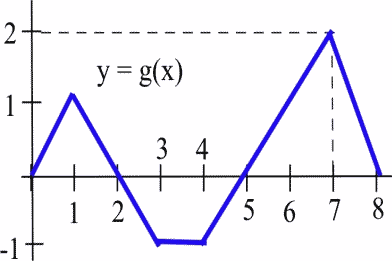
\includegraphics{images/image035.png}
\caption{}
\end{figure}

First, notice how to find the fixed cost and variable cost from the
graph here. FC is the \textbackslash{}(y\textbackslash{})-intercept of
the TC graph. (\textbackslash{}(FC = TC(0)\textbackslash{}).) The graph
of TVC would have the same shape as the graph of TC, shifted down.
(\textbackslash{}(TVC = TC - FC\textbackslash{}).)

\textbackslash{}(MC(q) = TC(q + 1) - TC(q)\textbackslash{}), but that's
impossible to read on this graph. How could you distinguish between
TC(4022) and TC(4023)? On this graph, that interval is too small to see,
and our best guess at the secant line is actually the tangent line to
the TC curve at that point. (This is the reason we want to have the
derivative definition handy.)

\textbackslash{}(MC(q)\textbackslash{}) is the slope of the tangent line
to the TC curve at \textbackslash{}( (q, TC(q))\textbackslash{}).

\textbackslash{}(MR(q)\textbackslash{}) is the slope of the tangent line
to the TR curve at \textbackslash{}((q, TR(q))\textbackslash{}).

Profit is the distance between the TR and TC curve. If you experiment
with a clear ruler, you'll see that the biggest profit occurs exactly
when the tangent lines to the TR and TC curves are parallel. This is the
rule ``profit is maximized when \textbackslash{}( MR =
MC\textbackslash{})'' which we'll explore later in the chapter.

\hypertarget{example-12}{%
\paragraph{Example 12}\label{example-12}}

The demand, \textbackslash{}(D\textbackslash{}), for a product at a
price of \textbackslash{}(p\textbackslash{}) dollars is given by
\textbackslash{}( D(p)=200-0.2p\^{}2 \textbackslash{}). Find the
marginal revenue when the price is \$10.

First we need to form a revenue equation. Since Revenue =
Price\textbackslash{}( \textbackslash{}times \textbackslash{})Quantity,
and the demand equation shows the quantity of product that can be sold,
we have \textbackslash{}{[}R(p)=D(p)\textbackslash{}cdot
p=\textbackslash{}left(200-0.2p\^{}2\textbackslash{}right)p=200p-0.2p\^{}3.\textbackslash{}{]}

Now we can find marginal revenue by finding the derivative:
\textbackslash{}{[}R'(p)=200(1)-0.2(3p\^{}2)=200-0.6p\^{}2\textbackslash{}{]}

At a price of \$10, \textbackslash{}( R'(10)=200-0.6(10)\^{}2=140
\textbackslash{}).

Notice the units for \textbackslash{}(R'\textbackslash{}) are
\textbackslash{}(\textbackslash{}frac\{\textbackslash{}text\{dollars of
Revenue\}\}\{\textbackslash{}text\{dollar of price\}\}\textbackslash{}),
so \textbackslash{}( R'(10)=140 \textbackslash{}) means that when the
price is \$10, the revenue will increase by \$140 for each dollar that
the price was increased.

\begin{longtable}[]{@{}ll@{}}
\toprule
\endhead
\href{section2-2.php}{← Previous Section} & \href{section2-4.php}{Next
Section →}\tabularnewline
\bottomrule
\end{longtable}
